\documentclass[aspectratio=43,display]{beamer}


\mode<presentation>
{
	\usetheme{Montpellier}	% or try Darmstadt, Madrid, Warsaw, ...
	\usecolortheme{rose}	% or try albatross, beaver, crane, dove...
	\usefonttheme{default}  % or try serif, structurebold, ...
	\setbeamertemplate{navigation symbols}{}
	\setbeamertemplate{caption}[numbered]
} 

\usepackage[english]{babel}
\usepackage[utf8x]{inputenc}
\usepackage{siunitx}
\usepackage{enumerate}
\usepackage{hyperref}
\usepackage{eso-pic}
\hypersetup{
	bookmarksopen=false,
	pdfpagemode=UseNone,
	%pdfpagemode=FullScreen,   %% Enable to have Adobe Reader query for fullscreen mode
	pdfauthor={Yuelin Xin} %% Enter the apppropriate author in here
}

\newcommand\AtPagemyUpperLeft[1]{\AtPageLowerLeft{%
		\put(\LenToUnit{0.75\paperwidth},\LenToUnit{0.9075\paperheight}){#1}}}
\AddToShipoutPictureFG{
	\AtPagemyUpperLeft{{
\includegraphics[width=3cm,keepaspectratio]{images/mf.png}}}
}%


\title[Scene Separation \& Data Selection]{Scene Separation \& Data Selection: Temporal Segmentation Algorithm for Real-time Video Stream Analysis}
%% Author with both abbreviation and affiliation
\author[YX, ZZ, YX]{Yuelin Xin\inst{1}\inst{2} \and Zihan Zhou\inst{1}\and Yuxuan Xia\inst{1}}
\institute[UL]{\inst{1}SWJTU-Leeds Joint School, CS\\Southwest Jiaotong University
	\and\inst{2}School of Computing\\University of Leeds}
\date[2022 STRL]{Spatio-Temporal Reasoning and Learning, 2022}


\begin{document}

	\begin{frame}
		\titlepage
	\end{frame}

	% Uncomment these lines for an automatically generated outline.
	\begin{frame}{Outline}
		\tableofcontents
	\end{frame}

	\section{Introduction}

		\begin{frame}{Introduction}

			\begin{itemize}
				\item The problem (Background \& What we want to achieve)
				\item Our motivation (Why not neural networks?)
			\end{itemize}

			\vskip 1cm

			\begin{block}{Remark}
				\textbf{Scene separation}(Temporal segmentation) is a problem in which we want to separate a video stream into different scenes.
				\textbf{A scene} is defined as a group of similar-looking frames that are temporally adjacent to each other.
			\end{block}

		\end{frame}


	\subsection{The problem}

		\begin{frame}{The problem}


			\begin{itemize}
				\item \textbf{Background}: real-time video stream interpretation, including video semantics / video accessibility / surveillance footage auto-interpretation, etc.
				\item \textbf{Difficulties}: algorithms do not see video as a continuous stream of images, but as discrete frames.
			\end{itemize}

			\vskip 0.3cm

			\begin{figure}
				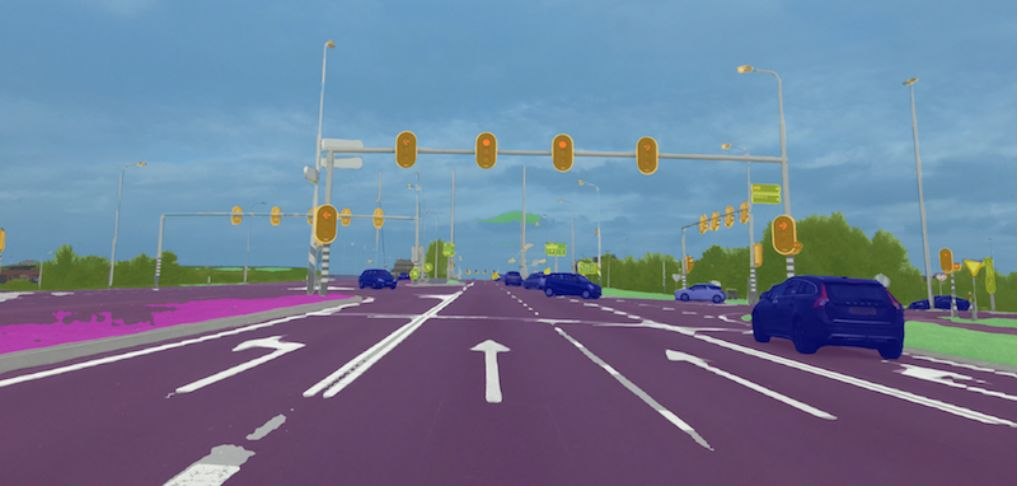
\includegraphics[width=5cm]{images/image-semantics.jpeg}
				\caption{\label{fig:Video-Semantics}Video semantics.}
			\end{figure}

		\end{frame}


		\begin{frame}{The problem}

			\begin{itemize}
				\item \textbf{The traditional approach}: 3D CNNs (CNN models with the additional temporal dimension)
				\item \textbf{What's missing}: hard to control when the video is very long or it is of indefinite length (like live streaming).
			\end{itemize}

			\vskip 0.5cm

			\begin{block}{Example}
				It would be hard to pick up sudden moves in long videos because the longer the video, the worse the temporal resolution.
				(like a very tiny object in a very massive picture in 2D CNNs)
			\end{block}

		\end{frame}


	\subsection{Our motivation}

		\begin{frame}{Our motivation}

			\textbf{Why not neural networks?}

			\begin{itemize}
				\item Neural networks are relatively slow, the inference time of a lot of NNs makes them difficult to be used in real-time video analysis.
				\item And the 2SDS algorithm is fully capable of handling simple scene separation tasks.
			\end{itemize}

			\vskip 0.3cm

			\begin{table}
				\centering
				\begin{tabular}{l|r|r}
				Algorithm & FPS(higher better) & Avg. Inference time\\\hline
				YOLOv5s & 11 & 92.2ms \\
				2SDS & 227 & 4.4ms
				\end{tabular}
			\caption{\label{tab:Speed-Comparision}Comparison of inference speed under same hardware.\footnote{Apple M1 (CPU)}}
			\end{table}

		\end{frame}


	\section{Method: 2SDS}

		\begin{frame}{Method: 2SDS}

			\begin{itemize}
				\item Related work: SlowFast Networks architecture
				\item Our work: 2SDS architecture
				\item Scene separation
				\item Data selection
			\end{itemize}

		\end{frame}

		\subsection{Related work}

			\begin{frame}{Related work}

				SlowFast Networks [Feichtenhofer \textit{et al}., 2019]

				\begin{itemize}
					\item \textbf{Slow pathway}:CNN with high spatial resolution(low FPS).
					\item \textbf{Fast pathway}:CNN with high temporal resolution(high FPS).
				\end{itemize}

				\begin{figure}
					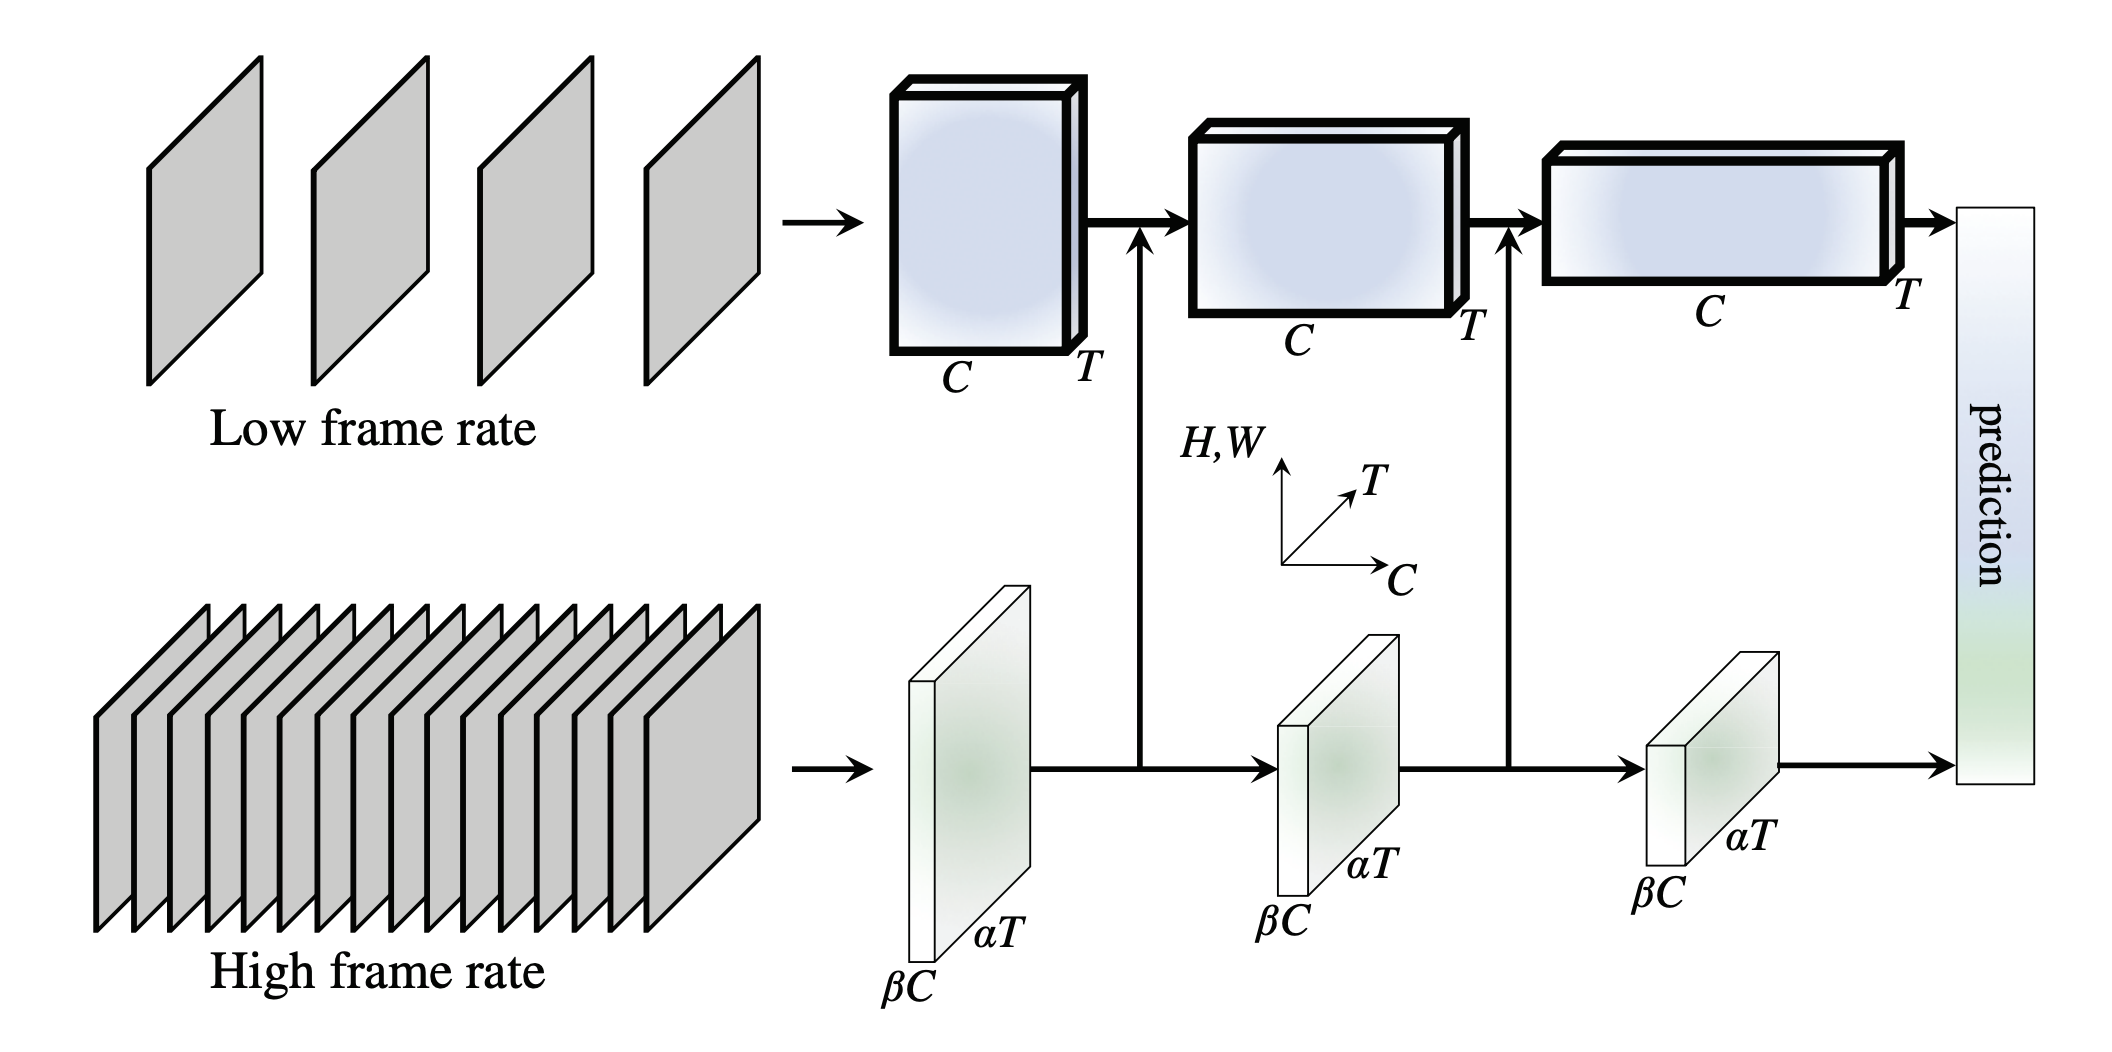
\includegraphics[width=7cm]{images/slowfast-networks.png}
					\caption{\label{fig:SlowFast-Networks}SlowFast Networks Architecture.}
				\end{figure}

			\end{frame}

		\subsection{Our work}
		
			\begin{frame}{Our work}

				Similar with the SlowFast Networks architecture, but we replace the fast pathway with 2SDS. \\
				This architecture has an even \textbf{finer temporal resolution} because we replaced the CNN with a faster algorithm.

				\vskip 0.2cm

				\begin{figure}
					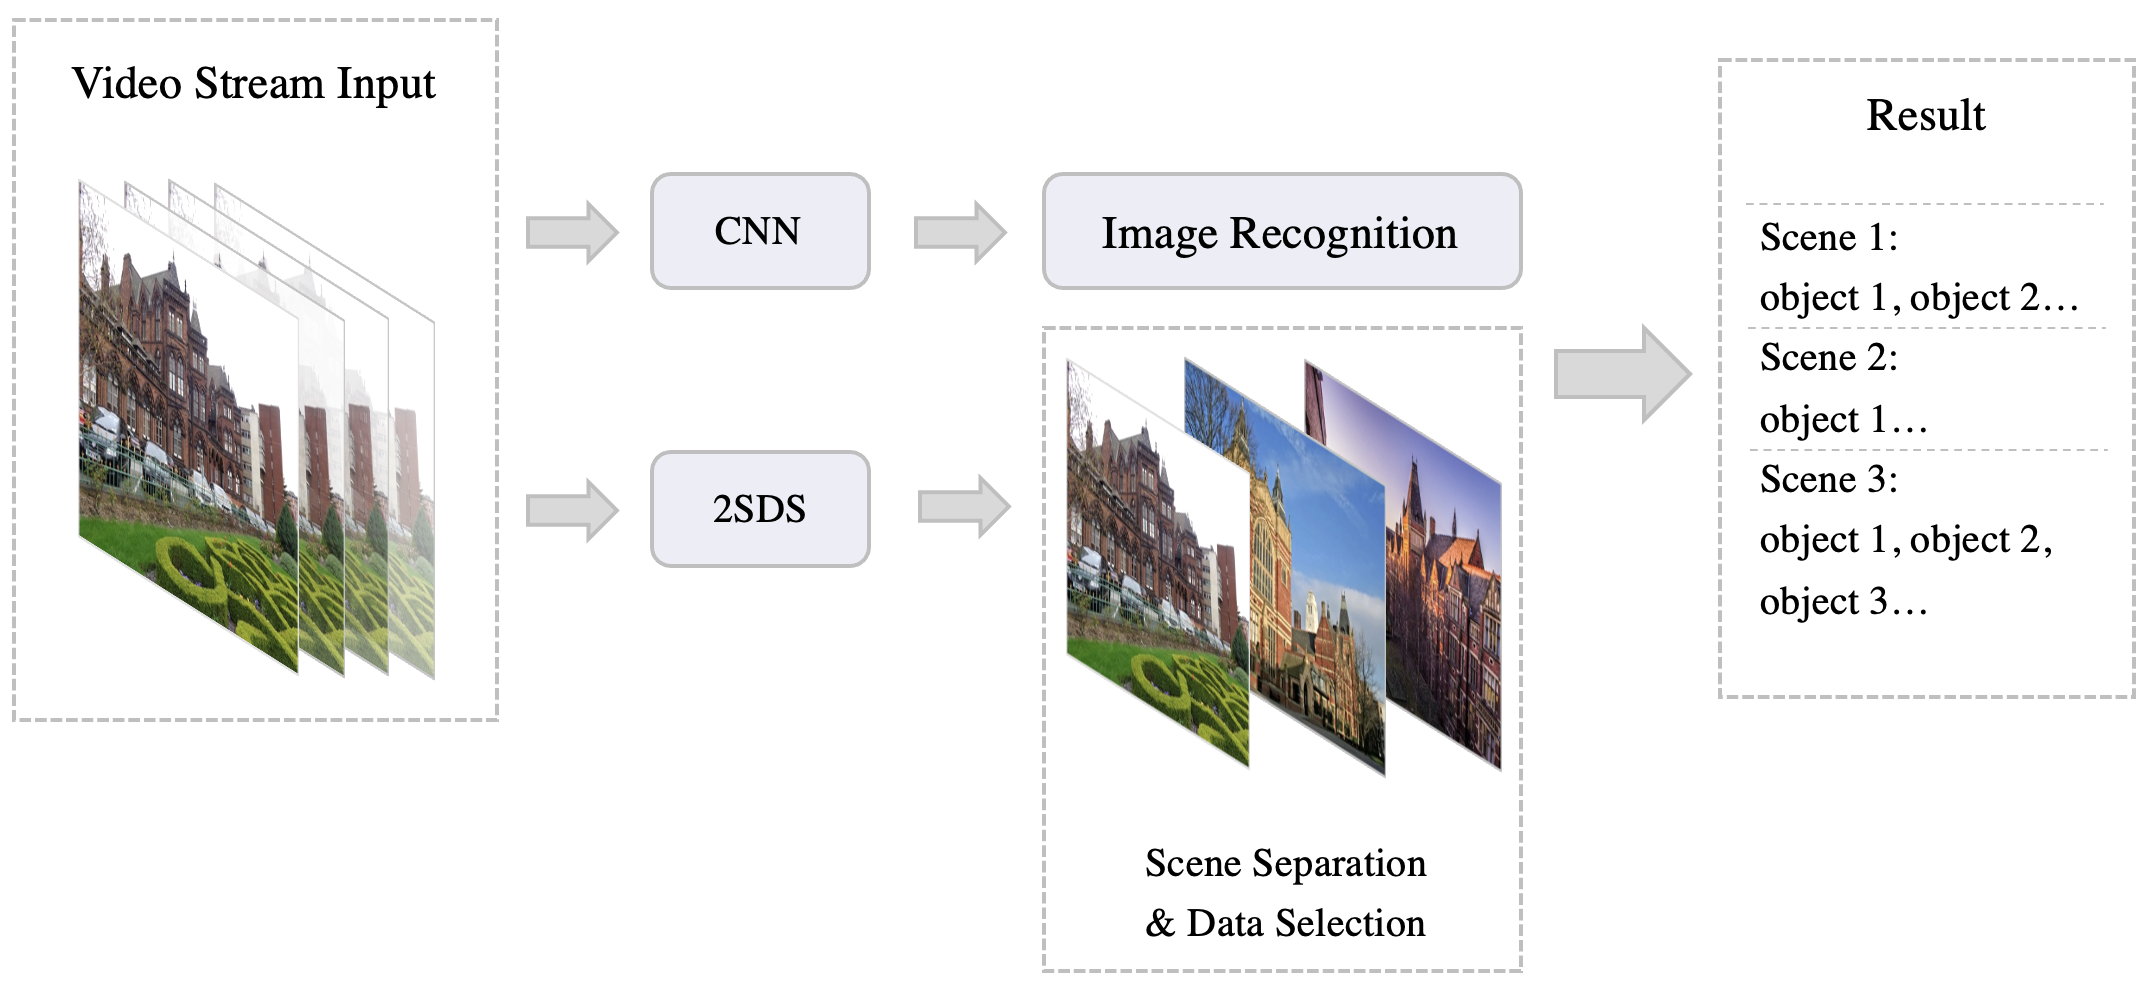
\includegraphics[width=7cm]{images/2SDS.png}
					\caption{\label{fig:2SDS}2SDS Architecture.}
				\end{figure}

			\end{frame}

			\begin{frame}{2SDS: a two step method}

				\begin{itemize}
					\item Step 1: \textbf{Scene separation}(Temporal segmentation)
					\item Step 2: \textbf{Data selection}
				\end{itemize}

			\end{frame}

		\subsection{Scene separation}

			\begin{frame}{Scene separation}

				\begin{itemize}
					\item \textbf{Down sample}: Downsample the frames to 8 by 9 
					(simplify calculation / make the algorithm less sensitive to small changes in the video).
					\item \textbf{Gray scale}: Convert RGB into grayscale to reduce calculation complexity.
				\end{itemize}

				\begin{figure}
					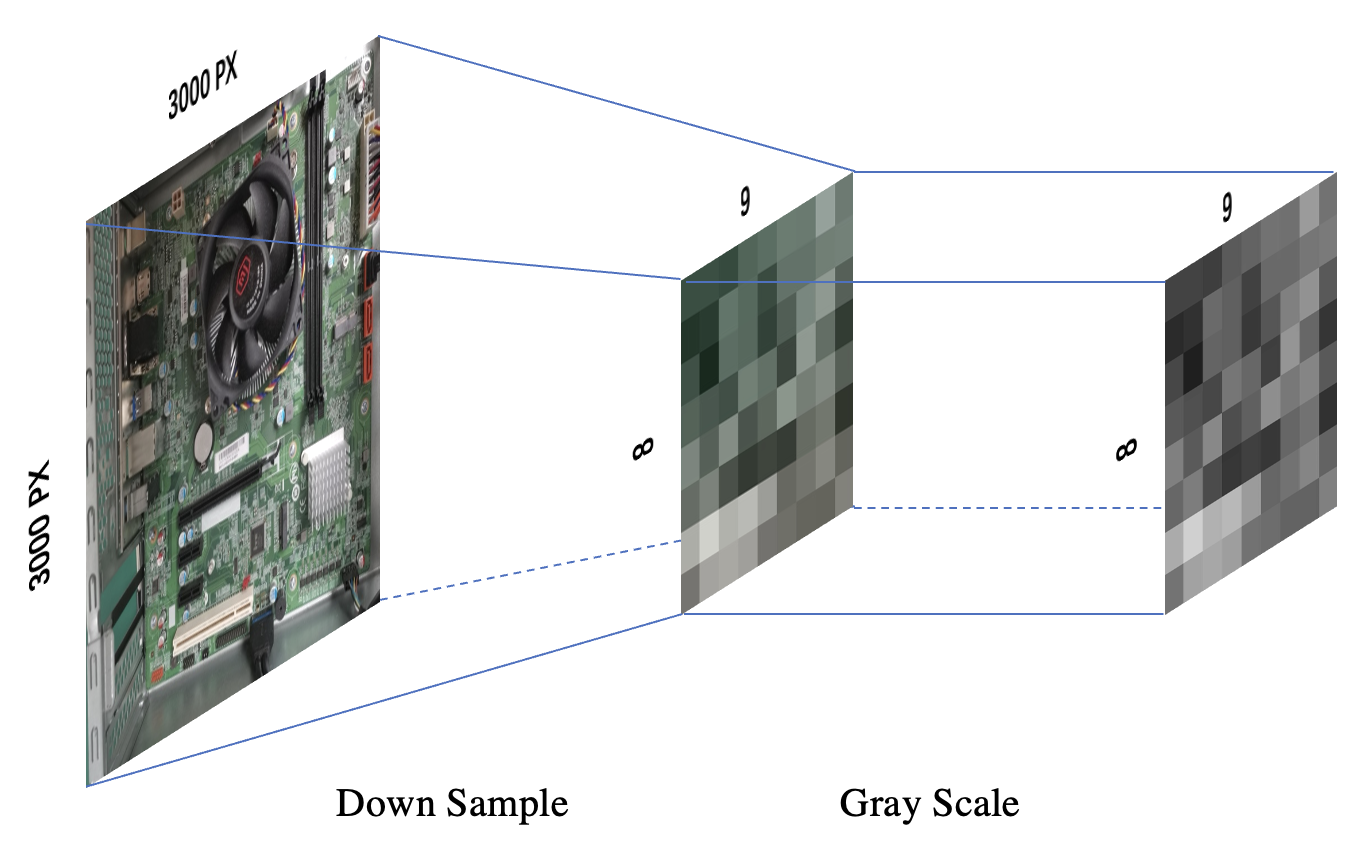
\includegraphics[width=5.5cm]{images/down-sample-grayscale.png}
					\caption{\label{fig:Scene-Separation}Temporal segmentation.}
				\end{figure}

			\end{frame}

			\begin{frame}{Scene separation}

				\begin{itemize}
					\item \textbf{Calculate Hash value}: Convert the grayscale graph into a 16-bit hash value, using the following rules:\\
					(a): One binary value stands for the grayscale difference between two adjacent pixels.\\
					(b): If the gray scale value of the pixel on the left is greater than the pixel on the right, the value is 1, otherwise it is 0.
				\end{itemize}

				\begin{figure}
					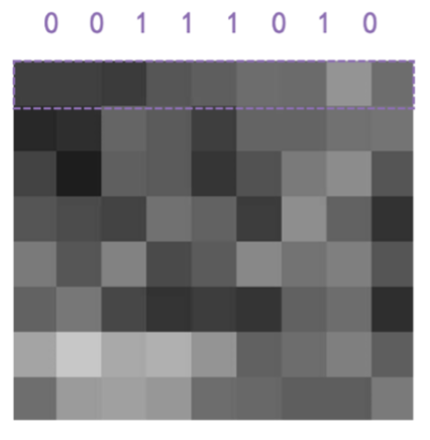
\includegraphics[width=2.5cm]{images/binary-sequence.png}
					\caption{\label{fig:Binary-Sequence}Binary sequence convertion.}
				\end{figure}
				
			\end{frame}

			\begin{frame}{Scene separation}

				\begin{itemize}
					\item \textbf{Calculate Hamming distance}: Calculate the Hamming distance between two adjacent frames.\\
					Hamming distance is what determines the similarity between two frames, the higher the distance, the less similar the two frames are.
				\end{itemize}

				\vskip 0.5cm

				\begin{block}{Example}
					The Hamming distance between the hash values $h_1=c4e0d8988c989898$ and $h_2=eee6989c8c989898$ is:	
					$ c4e0d8988c989898 \bigoplus eee6989c8c989898 = 7 $
				\end{block}
			
			\end{frame}

		\subsection{Data selection}

			\begin{frame}{Data selection}
				
				\begin{itemize}
					\item \textbf{Data smoothing}: Filter out the data noise by using a weighted average pooling filter.\\
					$$ \psi = \frac{\sum_{i=1}^{i\leqslant\varphi} (L_i \times \omega_i) }{\sum_{i=1}^{i\leqslant\varphi} \omega_i} $$\\
					$$ 
					    \left\{
							\begin{array}{ll}
								f_i(D) = \min_{i=0} |card(D_i) - \psi| \\
								C_I = [c \in D | card(c) = f_i(D) ]
							\end{array}
						\right. 
					$$
					\item \textbf{Data selection}: Merge the selected frames into a single frame(used as the output).
				\end{itemize}

			\end{frame}


	\section{Our results}

		\begin{frame}{Experiment}

			We have chosen 3 types of testing videos:

			\begin{itemize}
				\item \textbf{Interview}: relatively stationary, direct and clear.
				\item \textbf{Vibrant}: with a lot of movement and camera shifts.
				\item \textbf{Hybrid}: sometimes stationary, sometimes moving.
			\end{itemize}

		\end{frame}

		\begin{frame}{Preliminary results}

			\begin{table}
				\centering
				\begin{tabular}{l c r r}
					\hline
					Type No. & Output - Truth & Accuracy & 2SDS FPS  \\
					\hline
					Interview 1 & 25 - 25 & 100.00\% & \\
					Interview 2 & 35 - 29 & 82.86\% & \\
					Interview 3 & 31 - 28 & 90.32\% & \\
					Interview Avg. & 91 - 82 & 90.10\% & \\
					\hline
					Vibrant 1 & 9 - 13 & 69.23\% & \\
					Vibrant 2 & 19 - 38 & 50.00\% & \\
					Vibrant Avg. & 28 - 51 & 54.90\% & \\
					\hline
					Hybrid 1 & 105 - 106 & 99.06\% & \\
					\hline
				\end{tabular}
			\caption{\label{tab:Results}Preliminary experiment results.}
			\end{table}

		\end{frame}


	\section{Future improvements}

		\begin{frame}{Future improvements}



		\end{frame}


	\section{Conclusion}

		\begin{frame}{Conclusion}



		\end{frame}

\end{document}
